\section{Auswertung}
\label{sec:Auswertung}

\subsection{Kallibration und Bestimmung der Effizienz}
\label{subsec:a1}
Um das Energiespektrum für unbekannte Strahler sinnvoll interpretieren zu können,
ist eine Kalibrierung der Energieskala notwendig. Dazu wird das linienreiche Spektrum eines Europium 152 Strahlers betrachtet, welches in Abbildung \ref{fig:spektrum_eu} dargestellt ist.
\begin{figure}
 \centering
 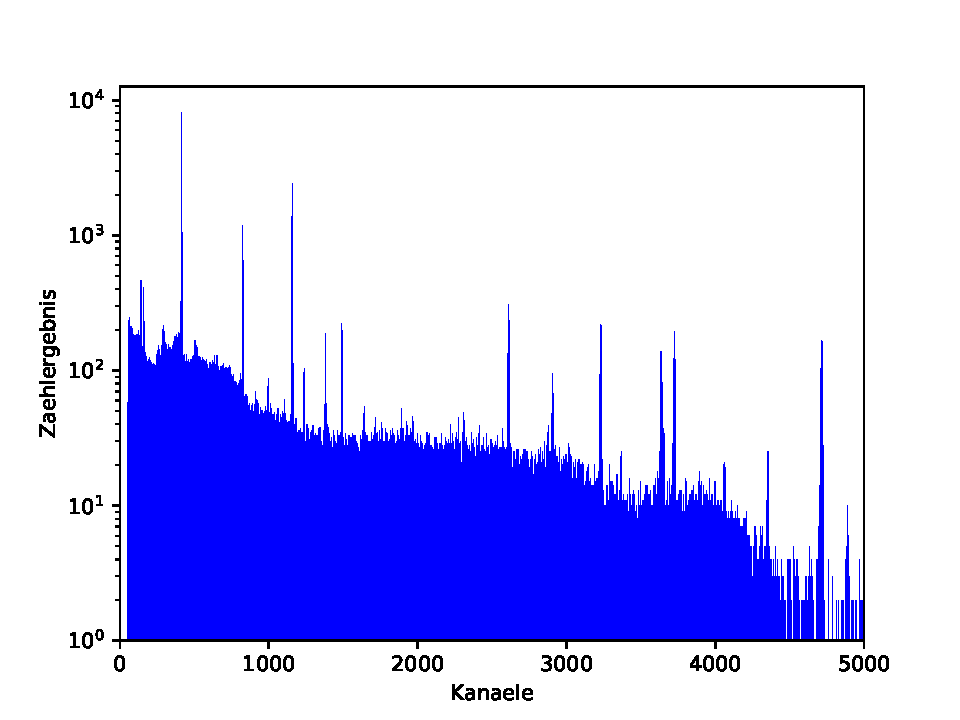
\includegraphics[width=0.8\textwidth]{python/plots/spec1.pdf}
 \caption{Rohdaten der Vermessung des Europium 152 Spektrums.}
 \label{fig:spektrum_eu}
 \end{figure} 
Um die Lage der Spektrallinien zu bestimmen wird zunächst ein Kanal, der als Position für eine Spektrallinie in Frage kommt, aus den Messdaten ausgelesen. 
Um diesen vorläufigen Kanal herum wird über die jeweils 20 oberhalb und unterhalb liegenden Kanäle eine Gauß-Funktion
\begin{align}
g(k)=c_1\exp\left(-c_2(k-c_3)^2\right)+c_4
\end{align}
an die Messdaten gefittet.
Dabei entspricht $c_1$ der Höhe der Spektrallinie und $c_3$ ihrer Lage.
Die Formel
\begin{align}
\int_\infty^\infty c_1\exp\left(-c_2(k-c_3)^2\right) dk = c_1 \sqrt{\frac{\pi}{c_2}}
\end{align}
zeigt, dass $c_2$ ein Maß für den Inhalt einer Spektrallinie ist.
Der Parameter $c_4$ dient dazu Störeffekte wie das Compton-Kontinuum oder die Untergrundstrahlung aus den folgenden Rechnungen zu eliminieren.
Er wird deshalb bei den folgenden Rechnungen nicht weiter berücksichtigt.
Diese und jede weitere Regressionsrechnung in dieser Auswertung wird mithilfe der Funktion \textit{curve\_ fit} aus dem Python Paket \textit{scipy.optimize} durchgeführt.
Die in Tabelle \ref{tab:atab1} angegebenen Kanäle werden in Abbildung \ref{fig:Kalibrierung} gegen die Literaturwerte des Eu-Spektrums aufgetragen. 
\begin{table}
\centering
\caption{Literaturwerte und gemessene Kanäle eines Europium 152 Gammaspektrums \cite{sample}.}
\begin{tabular}{c c c}
\hline \\
Kanal $k$ &Energie $E_\gamma$ in eV & Emissionswahrscheinlichkeit $W$ in \% \\
\hline \\
414.12 & 121.78 & 28.60 \\ 825.86 & 244.70 & 7.60 \\ 997.32 & 295.94 & 0.40 \\ 1158.71 & 344.30 & 26.50 \\ 1382.31 & 411.12 & 2.20 \\ 1491.59 & 443.96 & 3.10 \\ 2273.21 & 678.00 & 2.00 \\ 2310.43 & 688.67 & 0.90 \\ 2612.36 & 778.90 & 12.90 \\ 2908.55 & 867.37 & 4.20 \\ 3231.22 & 964.08 & 14.60 \\ 3368.59 & 1005.30 & 0.60 \\ 3639.40 & 1085.90 & 10.20 \\ 3726.07 & 1112.10 & 13.60 \\ 4353.21 & 1299.10 & 1.60 \\ 4716.58 & 1408.00 & 21.00 \\ 4888.94 & 1457.60 & 0.50 \\ 
\hline
\end{tabular}
\label{tab:atab1}
\end{table}
Über eine lineare Ausgleichsrechnung wird die Umrechnungsvorschrift
\begin{align*}
k(E) = s \cdot E + b \text{, mit}\\
  s = \SI{3.346+-0.001}{\per\electronvolt}\\
  b = \SI{ 5.9+-0.8}{}
\end{align*}
zwischen Kanalnummern und Energien in eV bestimmt.
\begin{figure}
\centering
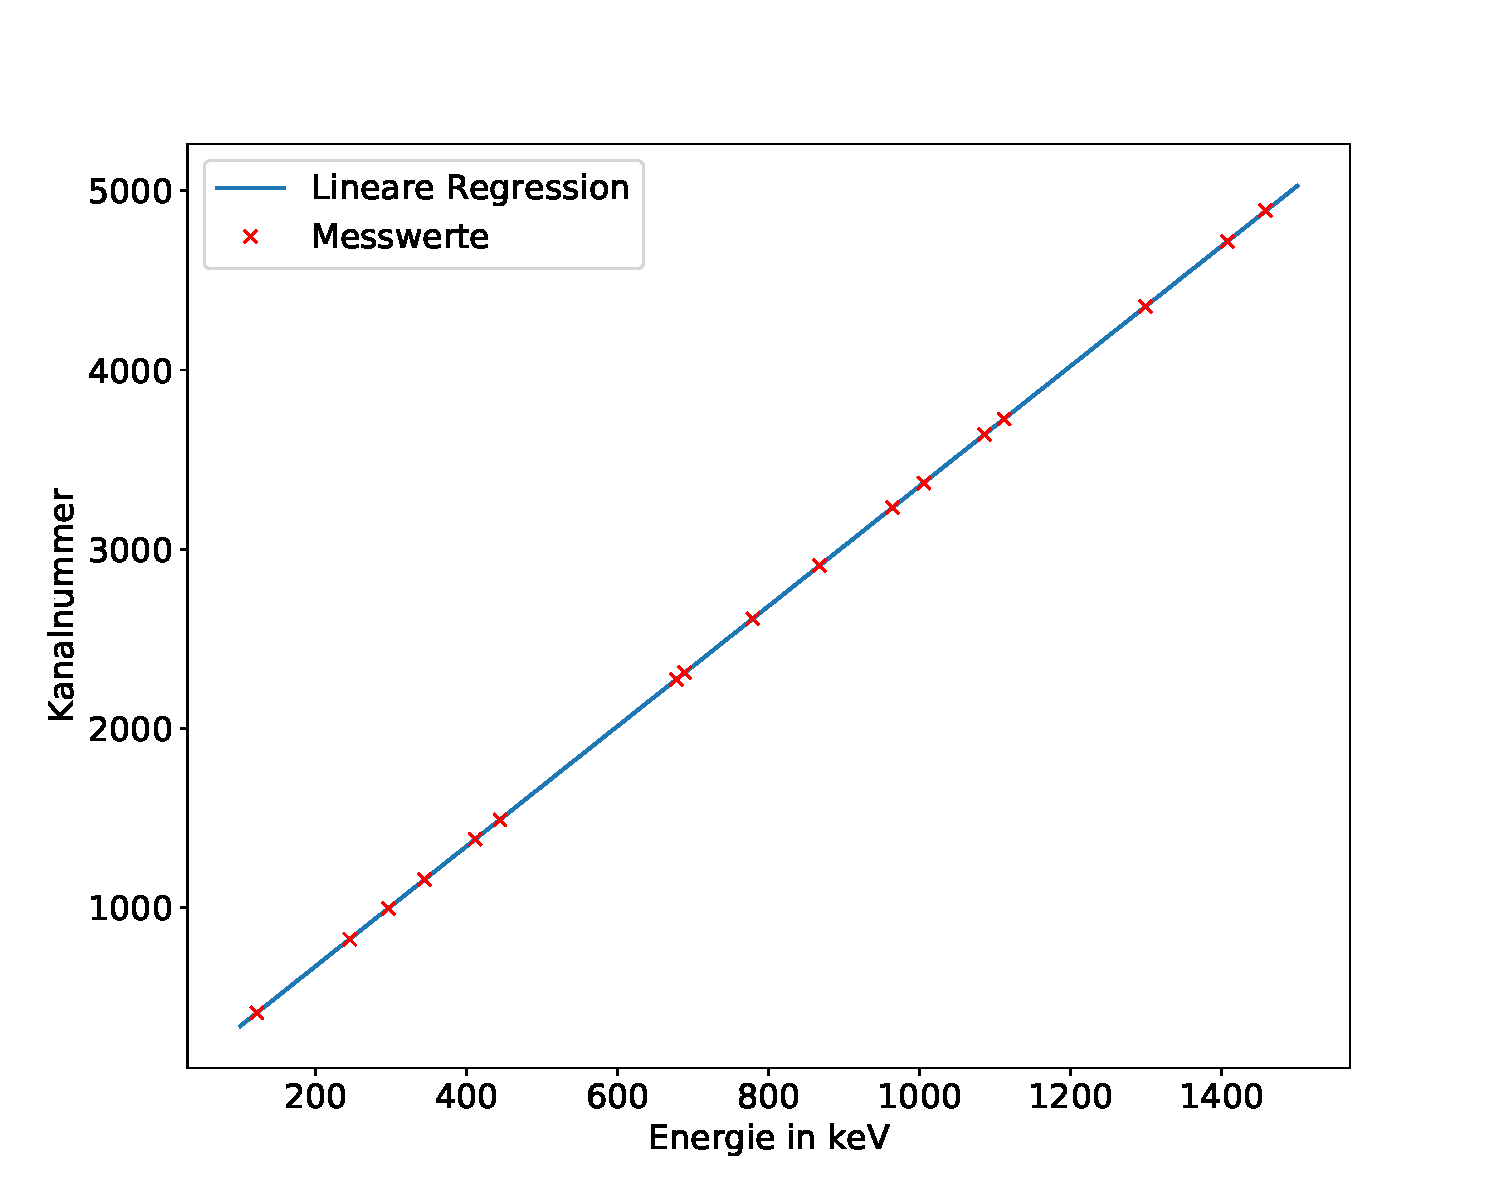
\includegraphics[width=0.8\textwidth]{python/plots/kalibrierung.pdf}
\caption{Lineare Regression der Messwerte aus Tabelle \ref{tab:atab1}}
\label{fig:Kalibrierung}
\end{figure}
Mit Gleichung \eqref{eqn:anleitung22} soll die Effizienz der Spektrallinien berechnet werden.
Um die dazu nötige Aktivität des Europiums zum Zeitpunkt der Messung zu bestimmen, wird das exponentielle Zerfallsgesetz
\begin{align}
A_\text{Messung}=A_0\exp\left(\frac{\log(2)}{T_{\frac{1}{2}}}\Delta t\right)
\end{align}
verwendet.
Die Aktivität $A_0$ am 01.10.2000 betrug $\SI{130+-60}{\becquerel}$ und die Halbwertszeit von Europium beträgt $\SI{4943+-5}{\day}$ \cite{sample}.
Das angegebene Datum liefert eine zeitliche Differenz von $\Delta t=\SI{6084}{\day}$, sodass sich eine Aktivität von 
\begin{align*}
A_\text{Messung}=\SI{1760+-26}{\becquerel}
\end{align*}
ergibt.
Leider wurde der Abstand $d$ zwischen Probe und Detektor nicht gemessen. 
Der Wert von $d=\SI{8.8+-0.3}{\centi\meter}$ wird deshalb dem Protokoll einer befreundeten Gruppe entnommen \cite{abstand}.
Der Radius der Probe beträgt $r=\SI{2.25}{\centi\meter}$ \cite{sample}.
Aus
\begin{align}
\frac{\Omega}{4\pi}=\frac{1}{2}\left( 1- \frac{d}{\sqrt{d^2+r^2}}\right)
\end{align}
lässt sich dann der Raumwinkel $\Omega=\SI{1.96+-0.021}{}$ berechnen.
Mit diesem Wert und den aus den Gauß-Fits Flächeninhalten der Gauß-Funktionen lassen sich nun die in Tabelle \ref{tab:atab2} angegebenen Effizienzen berechnen.
Dabei ist zu Berücksichtigen, dass die Zählrate aus Formel \ref{eqn:anleitung22} gerade den Inhalten geteilt durch die Messdauer $t_\text{Messung}=\SI{7764}{\second}$ entspricht.
\begin{table}
\centering
\caption{Inhalte der Gauß-Fits und die daraus berechneten Effizienzen.}
\begin{tabular}{c c c}
\hline \\
Energie in $\SI{}{\electronvolt}$ & Inhalt & Effizienz\\
\hline \\
121.78 & 28310.39$\pm$90.22 & 45.52$\pm$0.68 \\ 244.70 & 4765.44$\pm$42.44 & 28.84$\pm$0.49 \\ 295.94 & 230.91$\pm$25.33 & 26.55$\pm$2.94 \\ 344.30 & 11695.71$\pm$71.84 & 20.30$\pm$0.32 \\ 411.12 & 736.19$\pm$21.84 & 15.39$\pm$0.51 \\ 443.96 & 1012.15$\pm$20.59 & 15.02$\pm$0.38 \\ 678.00 & 43.35$\pm$13.43 & 1.00$\pm$0.31 \\ 688.67 & 240.92$\pm$19.87 & 12.31$\pm$1.03 \\ 778.90 & 2320.90$\pm$35.98 & 8.27$\pm$0.18 \\ 867.37 & 642.42$\pm$28.95 & 7.03$\pm$0.33 \\ 964.08 & 2083.95$\pm$43.93 & 6.56$\pm$0.17 \\ 1005.30 & 90.85$\pm$13.17 & 6.96$\pm$1.01 \\ 1085.90 & 1166.39$\pm$39.80 & 5.26$\pm$.20 \\ 1112.10 & 1831.04$\pm$40.33 & 6.19$\pm$0.16 \\ 1299.10 & 160.40$\pm$16.65 & 4.61$\pm$0.48 \\ 1408.00 & 2293.51$\pm$65.45 & 5.02$\pm$0.16 \\ 1457.60 & 176.49$\pm$51.70 & 16.23$\pm$4.76\\
\hline
\end{tabular}
\label{tab:atab2}
\end{table}
Es wird angenommen, dass die Effizienz $Q$ mit steigender Energie wie eine Potenzfunktion
\begin{align}
Q(E)=c E^{d}
\end{align}
abnimmt.
Die in Abbildung \ref{fig:Effizienz} dargestellte Regressionsrechnung liefert die Parameter
\begin{align*}
c&=\SI{30+-10}{}
d&=\SI{-0.87+-0.08}{}\text{ .}
\end{align*}
\begin{figure}
\centering
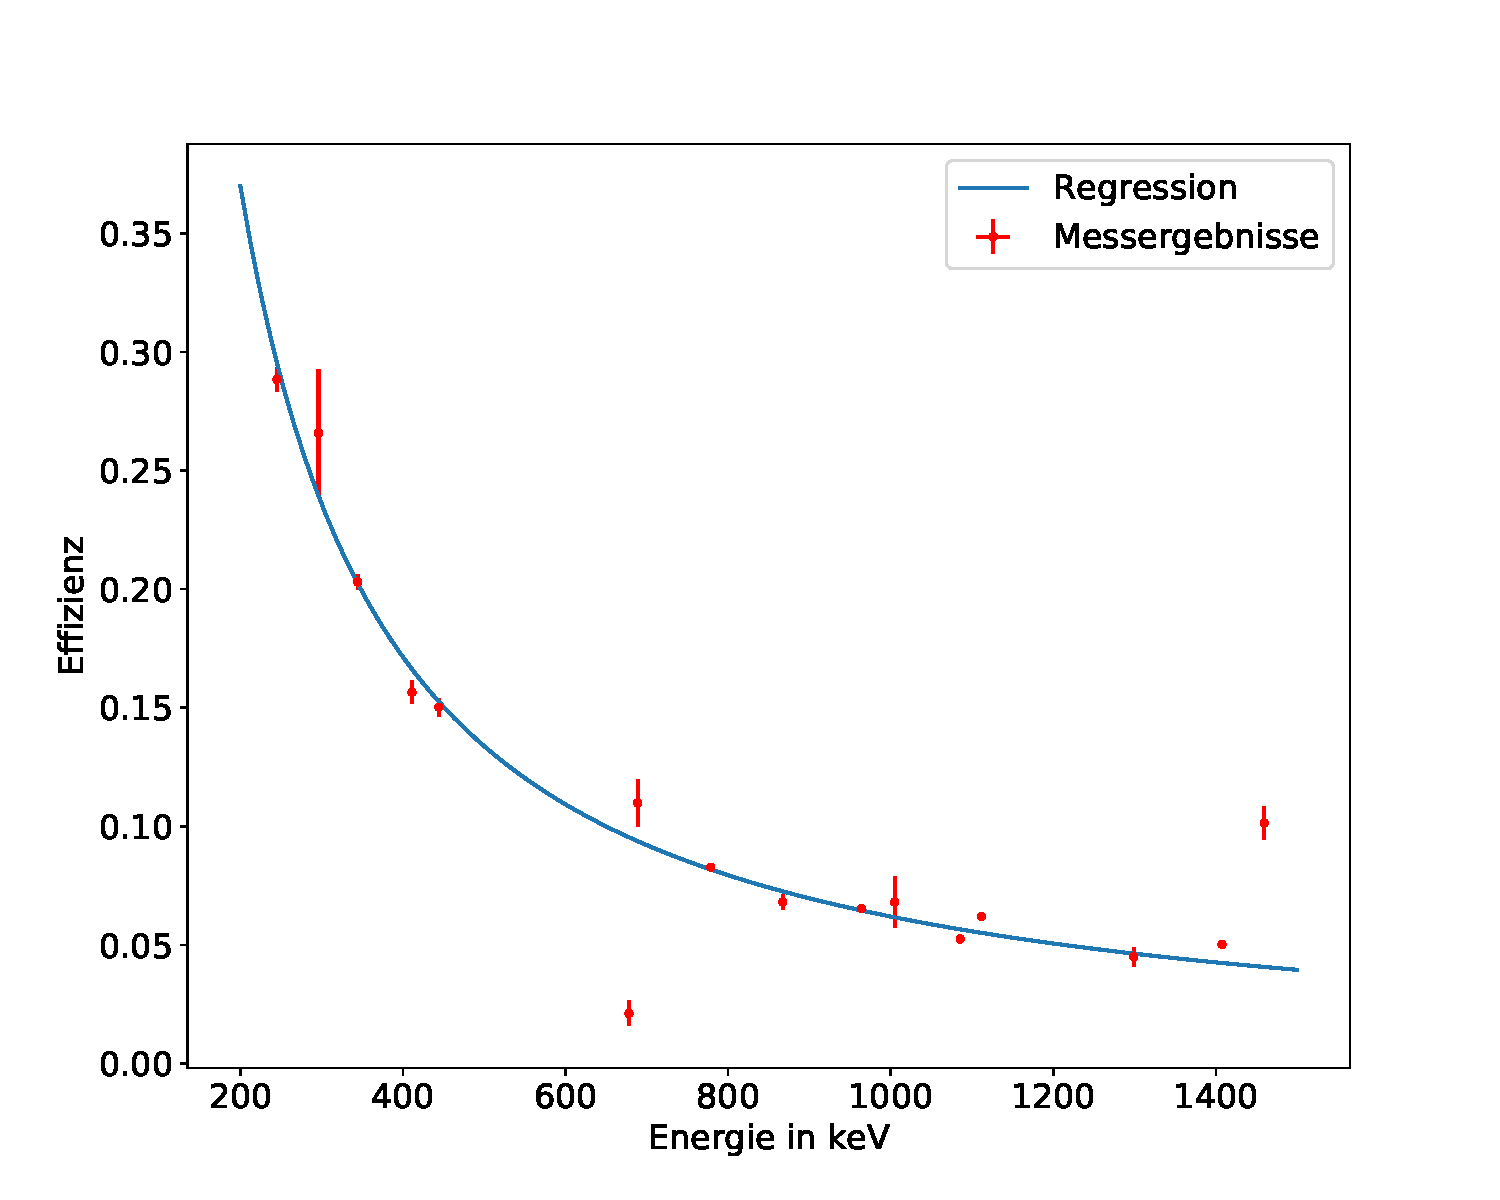
\includegraphics[width=0.8\textwidth]{python/plots/effizienz.pdf}
\caption{Darstellung der Abnahme der Effizienz mit Steigender Energie durch eine Regressionsrechnung. Energien unterhalb von $\SI{150}{\electronvolt}$ werden nicht betrachtet.}
\label{fig:Effizienz}
\end{figure}
\subsection{Bestimmungen von Detektoreigenschaften}
\label{subsec:a2}






\subsection{Aktivitätsbestimmung von }
\label{subsec:a3}

\subsection{Untersuchung von Zerfallsketten in }
\label{subsec:a4}



%\begin{figure}
%  \centering
%  \includegraphics{plot.pdf}
%  \caption{Plot.}
%  \label{fig:plot}
%\end{figure}
